\documentclass[12pt,a4paper]{article}

\usepackage[left=3cm, right=3cm, top=2.5cm, bottom=2.5cm]{geometry}
\usepackage{setspace}
\usepackage{amsmath}
\usepackage{tikz}
\usepackage{pgfplotstable}
\usepackage{titlesec}
\usepackage{bm}
\usepackage{tcolorbox}
\tcbuselibrary{skins}
\usepackage{empheq}
\usepackage{booktabs}
\usepackage{caption}
\usepackage{hyperref}
\usepackage{fancyhdr}
\hypersetup{
    colorlinks=true,
    linkcolor=black,
    filecolor=magenta,      
    urlcolor=cyan,
    pdfpagemode=FullScreen,
    }
\usepackage{graphicx}
\graphicspath{ {./images/} }


\titleformat{\section}{\Large\bfseries}{\thesection}{1em}{}
\titleformat{\subsection}{\large\bfseries}{\thesubsection}{1em}{}


\renewcommand{\contentsname}{Table des Matières}
\renewcommand{\tablename}{Tableau }
%\renewcommand{\baselinestretch}{1.5}

\title{Étude des équations balistiques}
\author{Liviu Arsenescu, Cătălin Bozan}
\date{date}

\newtcbox{\mymath}[1][]{%
    nobeforeafter,
    math upper,
    tcbox raise base,
    enhanced,
    colframe=black,
    colback=white,
    boxrule=1pt,
    drop shadow={
        shadow xshift=3pt,
        shadow yshift=-3pt,
        opacity=1
    },
    #1
}

\pagestyle{fancy}
\fancyhf{}
\rhead{
\includegraphics[width=4cm]{hearclogo.png}}
\lhead{\thepage}
\setlength{\headsep}{30pt}

\begin{document}
    \pagenumbering{gobble}
    \begin{titlepage}
        \begin{center}
            \vspace*{\fill}
            \Huge \textbf{Étude des équations de la balistique :} \\
            \Huge \textbf{Équations du mouvement dans un champ gravitationnel} \\
            \Large Rapport du Laboratoire \\
            \begin{figure}[h]
                \centering
                
\includegraphics[width=7cm]{hearclogo.png}
            \end{figure}
            \vspace{\fill}
            \Large Liviu Arsenescu, Cătălin Bozan \\
            19.03.2024

            \vspace*{\fill}
        \end{center}
    \end{titlepage}

    \thispagestyle{empty}
    \tableofcontents
    \newpage

    \pagenumbering{arabic}
    \section{Description de l'expérience}
    \subsection{Buts}
    \begin{itemize}
        \item Vérifier les équations de la balistique
        \item Obtenit la vitesse à laquelle le canon tire le boulet
        \item Pédire la hauteur de l'impact de la bille contre un mur avec un tir oblique
    \end{itemize}

    \subsection{Éléments théoriques}
    \subsubsection{Les différentes grandeurs physiques rencontrées}
    \begin{minipage}{0.6\linewidth}
        \begin{itemize}
            \item \textbf{h} - hauteur initiale 
            \item \textbf{d} - distance entre le canon et le point d'impact 
            \item \textbf{H} - hauteur d'impact
            \item $\bm{\theta}$ - angle de tir 
            \item $\bm{v_0}$ - vitesse de sortie du canon
            \item $\bm{g}$ - accélération gravitationnelle de Terre
        \end{itemize}
    \end{minipage}%
    \hfill
    \begin{minipage}{0.4\linewidth}
        \begin{itemize}
            \item[-] $\bm{[h]=m}$
            \item[-] $\bm{[d]=m}$
            \item[-] $\bm{[H]=m}$
            \item[-] $\bm{[\theta]=deg}$
            \item[-] $\bm{[v_0]=ms^{-1}}$
            \item[-] $\bm{g}=9.81ms^{-1}$
        \end{itemize}   
    \end{minipage}
    \subsubsection{Les équations de la balistique}
    Dans le cas du mouvement qui nous intéresse, on peut observer deux types de mouvements :
    \begin{enumerate}
        \item Mouvement à vitesse constante, avec l'équation :
        \begin{align*}
            x(t) = v_xt + x_0
        \end{align*}
        \item Mouvement à accélération constante, avec les équations :
        \begin{align*}
            v_x(t) &= a_xt + v_{x0} \\
            x(t) &= \frac{1}{2}a_xt^2 + v_x(t) + x_0
        \end{align*}
    \end{enumerate}
    Où $x(t)$ est le déplacement sur n'importe quel axe de nom x, en fonction du temps, $v_x(t)$ est la vitesse sur l'axe x et $a_x$ est l'accélération. \\
    Pour étudier le tir au canon, on a les contraintes mathématiques suivantes :
    \begin{equation*}
        \vec{v_0}=
        \begin{pmatrix}
            v_{x0} \\
            v_{y0}
        \end{pmatrix}, 
        \|\vec{v_0}\|=v_0
    \end{equation*}
    \begin{itemize}
        \item Pour l'axe x :
        \begin{align*}
            x_0 &= 0 \\
            v_x(t)&=v_0cos(\theta)
        \end{align*}
        \item Pour l'axe y :
        \begin{align*}
            a_y &= -g \\
            v_{y0} &= v_0sin(\theta) \\
            y_0 &= h
        \end{align*}
        Où :
        \begin{itemize}
            \item $v_0$ - vitesse de sortie du canon
            \item $\theta$ - angle entre $\vec{v_0}$ et l'axe x
            \item $g$ - accélération gravitationnelle de Terre
            \item $h$ - hauteur de départ
        \end{itemize}
    \end{itemize}
    Avec ces contraintes, on peut construire le système d'équations suivant pour le mouvement que on étudie :
    \begin{center}
        \vspace{-\baselineskip}
        \begin{minipage}{0.3\linewidth}
            \begin{empheq}[box={\mymath}]{align*}
                x(t) &= v_0cos(\theta)t \\
                v_x(t) &= v_0cos(\theta)
            \end{align*}
        \end{minipage}%
        \begin{minipage}{0.1\linewidth}
            \begin{center}
                et
            \end{center}
        \end{minipage}%
        \begin{minipage}{0.4\linewidth}
            \begin{empheq}[box={\mymath}]{align*}
                y(t) &= \frac{-1}{2}gt^2 + v_0sin(\theta)t + h \\
                v_y(t) &= -gv_0sin(\theta) + v_0sin(\theta)
            \end{align*}
        \end{minipage}
    \end{center}
    \subsubsection{Tir horizontal :}
    \begin{center}
        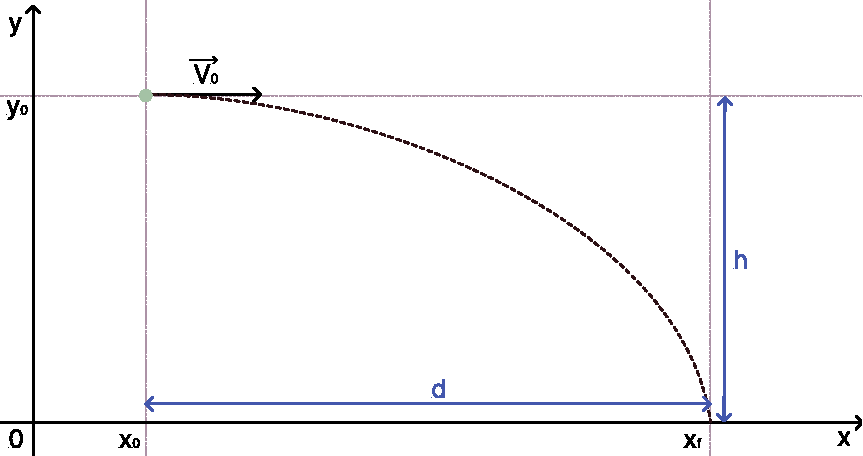
\includegraphics[scale=0.8]{exp1_graph.pdf} \\
    \end{center}
    Pour le tir horizontal, le vecteur vitesse fait avec l'axe x un angle $\theta$ de $0^\circ$ :
    \begin{align*}
        cos(\theta)=1&, sin(\theta)=0 \\
        \vec{v_0}=
        \begin{pmatrix}
            v_{x0} \\
            v_{y0}
        \end{pmatrix}
        =
        \begin{pmatrix}
            v_{x0} \\
            0
        \end{pmatrix}
        &\Rightarrow \|\vec{v_0}\|=v_{x0}=v_0,
    \end{align*}
    Pour la position initiale($\vec{r_0}$), on a les valeurs suivantes :
    \begin{equation*}
        \vec{r_0}=
        \begin{pmatrix}
            x_0 \\
            y_0
        \end{pmatrix}
        =
        \begin{pmatrix}
            0 \\
            h
        \end{pmatrix}
    \end{equation*}
    Nos équations deviennent :
    \begin{itemize}
        \item Pour l'axe x :
        \begin{empheq}[box={\mymath}]{align*}
            x(t)&=v_0t \\
            v_x(t)&=v_0
        \end{align*}
        \item Pour l'axe y
        \begin{empheq}[box={\mymath}]{align*}
            y&=-\frac{1}{2}gt^2+h \\
            v_y(t)&=-gt
        \end{align*}
    \end{itemize}
    L'instant où l'objet touche le sol nous donne la distance horizontale entre le point de départ et le point d'arrivée (d) :
    \begin{align*}
        y(t_f)=0 \Rightarrow& t_f=\sqrt{\frac{2h}{g}} \\
        x(t_f) = v_0\cdot t_f &= v_0 \cdot \sqrt{\frac{2h}{g}} \\
        \Downarrow
    \end{align*}
    \begin{empheq}[box={\mymath}]{equation*}
        d=v_o \cdot \sqrt{\frac{2h}{g}}
    \end{equation*}
    \subsubsection{Tir oblique :}
    \begin{center}
        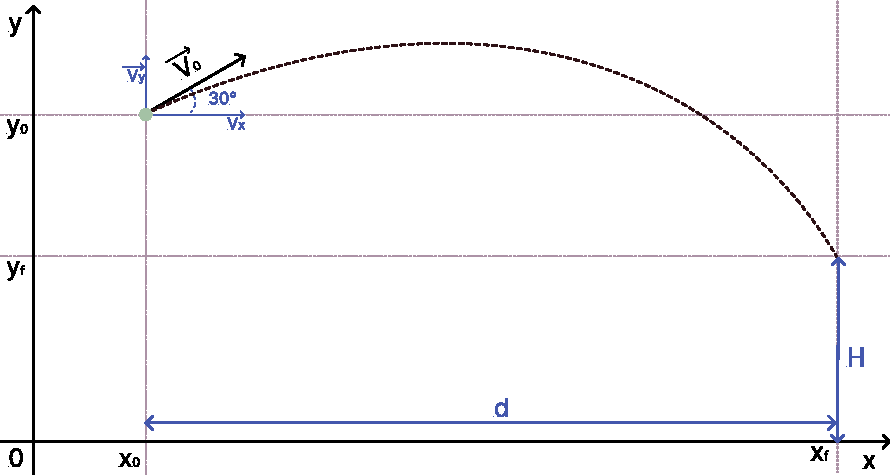
\includegraphics[scale=0.8]{exp2_graph.pdf} \\
    \end{center}
    Pour le tir oblique, le vecteur vitesse fait avec l'axe x un angle $\theta$ de $30^\circ$ :
    \begin{align*}
        cos(\theta)&=\frac{\sqrt{3}}{2},sin(\theta)=\frac{1}{2} \\
        \vec{v_0}=
        \begin{pmatrix}
            v_{x0} \\
            v_{y0}
        \end{pmatrix}
        &= 
        \begin{pmatrix}
            v_0cos(\theta) \\
            v_0sin(\theta)
        \end{pmatrix}
        =
        \begin{pmatrix}
            \frac{\sqrt{3}}{2}v_0 \\
            \frac{1}{2}v_0
        \end{pmatrix}
    \end{align*}
    Pour la position initiale($\vec{r_0}$), on a toujours valeurs :
    \begin{equation*}
        \vec{r_0}=
        \begin{pmatrix}
            x_0 \\
            y_0
        \end{pmatrix}
        =
        \begin{pmatrix}
            0 \\
            h
        \end{pmatrix}
    \end{equation*}
    Nos équations deviennent :
    \begin{itemize}
        \item Pour l'axe x :
        \begin{empheq}[box={\mymath}]{align*}
            x(t)&=v_0cos(\theta)t \\
            v_x(t)&=v_0cos(\theta)
        \end{align*}
        \item Pour l'axe y
        \begin{empheq}[box={\mymath}]{align*}
            y(t)&=-\frac{1}{2}gt^2+v_0sin(\theta)t+h \\
            v_y(t)&=-gt + v_0sin(\theta)
        \end{align*}
    \end{itemize}
    Comme on connaît la distance à laquelle le projectile frappe le mur (d), on peut aussi calculer la hauteur au même endroit (H).
    \begin{align*}
        x(t_f)&=d \Rightarrow t_f= \frac{d}{v_0cos(\theta)} \\
        y(t_f)&=-\frac{1}{2}gt_f^2 + v_0sin(\theta)t_f+h \\
        y(t_f)&=\frac{-g}{2} \frac{d^2}{cos^2(\theta)v_0^2} + tan(\theta)d+h \\
        &\Downarrow
    \end{align*}
    \begin{empheq}[box={\mymath}]{align*}
        H=\frac{-2}{3}\frac{d^2}{v_0^2}g &+ \frac{\sqrt{3}}{3}d+h
    \end{align*}

    \newpage
    \subsection{Principe de l'expérience}
    L'expérience va donc se dérouler en deux parties :
    \begin{enumerate}
        \item On a mesurer la distance à laquelle le projectile touche le sol, en utilisant differentes hauteurs de tir. On peut donc utiliser les valeurs mesurées (d et h) pour calculer la vitesse de tir du canon ($v_0$).
        \item On mesure pour 5 tirs obliques la hauteur où le projectile touche le mur pour obtenir une hauteur expérimentale $H_{exp}$. Après, on utilise la vitesse calculée lors de la première expérience pour calculer une hauteur attendue $H_{calc}$. En fin on compare les deux.
    \end{enumerate}
    \subsection{Schéma et montage de l’expérience}
    Pour réaliser l'expérience, on a besoin d'un dispositif qui lance une bille, d'un moyen de marquer avec précision l'endroit où la bille a atterri et d'un moyen pour changer la hauteur et l'angle du canon.
    Dans notre cas, on a utilisé :
    \begin{itemize}
        \item Un canon à ressort à angle variable
        \item Une bille en plastique
        \item Du papier
        \item Du papier carbone
        \item Des boîtes, sur lesquelles nous avons posé le canon pour changer la hauteur du canon.
    \end{itemize}  
    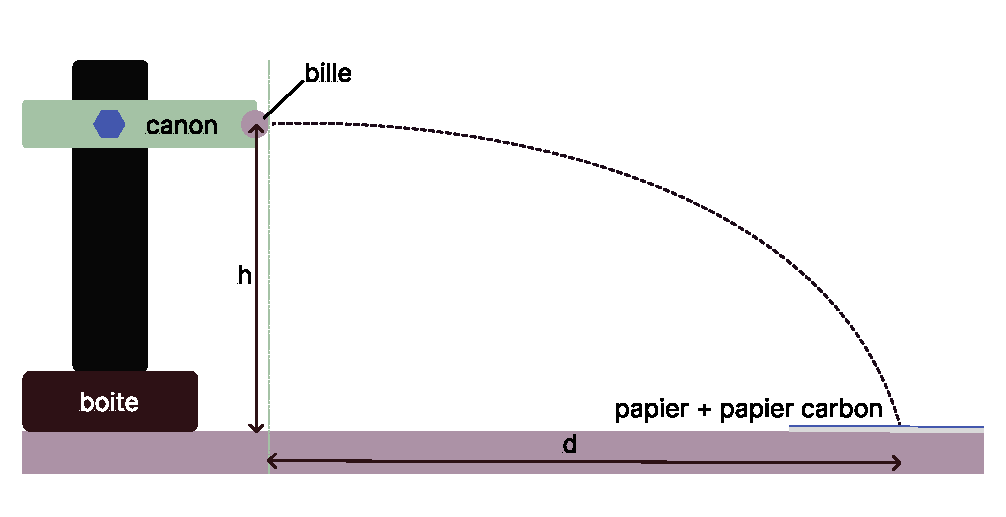
\includegraphics[width=0.4\paperwidth]{images/exp1_2.pdf}
    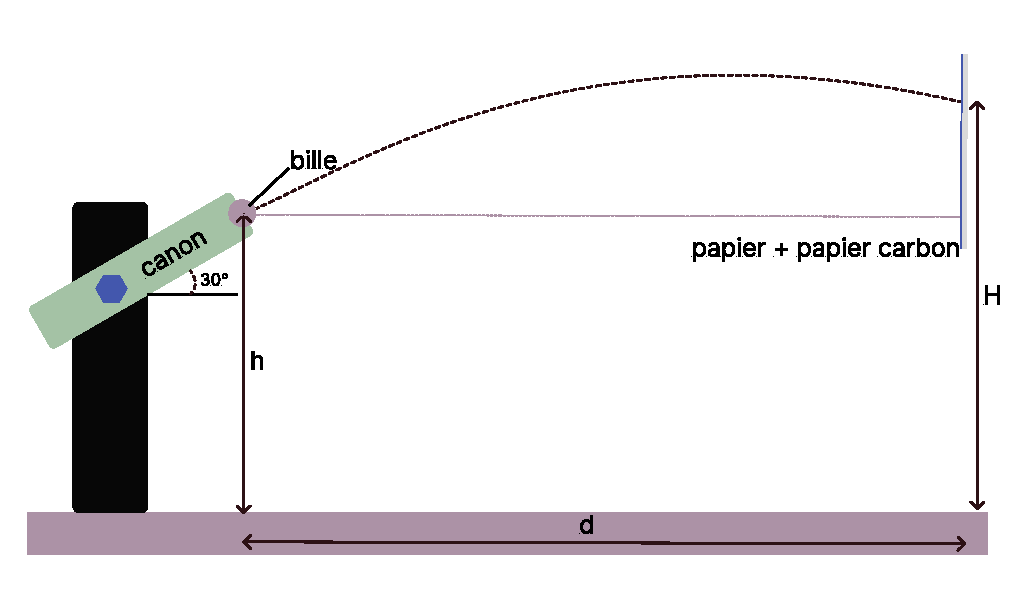
\includegraphics[width=0.4\paperwidth]{images/exp2_1.pdf}
    
    \subsection{Déroulement de l'expérience}
    \subsubsection{Tir horizontal : déduction la vitesse $v_0$ de sortie de la bille}
    \begin{itemize}
        \item Assurez-vous que le canon est réglé à un angle de zéro dégréé.
        \item Posez le canon sur le sol et tirez la bille en utilisant la puissance la plus faible du canon à ressort.
        \item Observez l'endroit où la bille a atterri et collez une feuille de papier sur le sol à l'endroit où la bille a atterri.
        \item Placez une feuille de papier carbone sur la feuille de papier.
        \item Tirez la bille cinq fois avec la même force de ressort afin de la faire tomber sur le papier carbone et de marquer sa position d'atterrissage.
        \item Mesurez la hauteur entre le sol et le bas de la marque de la bille sur le canon.
        \item Tracez des lignes perpendiculaires au canon qui passent par les marques laissées par la bille sur le papier carbone.
        \item Mesurer la distance entre les lignes perpendiculaires et la projection du centre de masse de la bille sur le sol.
        \item Utiliser des boîtes placées sous le canon pour modifier sa hauteur et répéter l'expérience pour 5 hauteurs différentes.
        \item Pour chaque hauteur, on calcule la vitesse du canon.
    \end{itemize}

    \subsubsection{Tir oblique : déduction de $H_{exp}$ et $H_{calc}$ sur le mur}

    \begin{itemize}
        \item Placer le canon à un angle de $30^\circ$.
        \item Placez le canon de manière à ce qu'il y ait une distance de 70 cm entre le mur et le point où la bille toucherait le mur.
        \item Tirez une bille avec la puissance la plus faible du canon et collez une feuille de papier sur le mur à l'endroit où la bille a atterri.
        \item Coller le papier carbone sur la feuille de papier.
        \item Tirez la bille 5 fois avec le même réglage du canon, à la puissance la plus faible.
        \item Mesurez la distance entre les marques laissées par la bille sur le papier et le sol pour pouvoir déduire $H_{exp}$.
        \item Utiliser la vitesse $v_0$ trouvée au point 1 pour calculer une hauter $H_{calc}$, comme valeur attendue.
    \end{itemize}

    \newpage
    \section{Mesures}
    \subsection{Tir horizontal :}
    \begin{table}[ht!]
        \centering
        \begin{tabular}{c|c|c|c|c|c|c|c}
            \toprule
             $h$(m) & $d_1$(m) & $d_2$(m) & $d_3$(m) & $d_4$(m) & $d_5$(m) & $\bar{d}$(m) & $\sigma_d$(m) \\
            \midrule
            0.149 & 0.711 & 0.761 & 0.771 & 0.787 & 0.749 & 0.756 & 0.029 \\
            0.361 & 0.842 & 0.844 & 0.910 & 0.924 & 0.844 & 0.873 & 0.041 \\
            0.475 & 0.944 & 0.976 & 0.987 & 1.018 & 0.979 & 0.981 & 0.026 \\
            0.587 & 1.115 & 1.127 & 1.134 & 1.138 & 1.164 & 1.136 & 0.018 \\
            0.701 & 1.135 & 1.156 & 1.169 & 1.183 & 1.225 & 1.174 & 0.034 \\
            \bottomrule
        \end{tabular}
        \caption{Mesures pour la première expérience}
    \end{table}
    \begin{table}[ht!]
        \centering
        \begin{tabular}{c|c|c|c|c|c}
            \toprule
             $h$(m) & $\Delta h$(m) & $\bar{d}$(m) & $\sigma_d$(m) & $\sqrt{\frac{2h}{g}}$(s) & $\Delta \sqrt{\frac{2h}{g}}$(s) \\
            \midrule
            0.149 & 0.003 & 0.756 & 0.029 & 0.174 & 0.004 \\
            0.361 & 0.003 & 0.873 & 0.041 & 0.271 & 0.002 \\
            0.475 & 0.003 & 0.981 & 0.026 & 0.311 & 0.002 \\
            0.587 & 0.003 & 1.136 & 0.018 & 0.346 & 0.002 \\
            0.701 & 0.003 & 1.174 & 0.034 & 0.378 & 0.002 \\
            \bottomrule
        \end{tabular}
        \caption{Mesures pour la première expérience (régression linéaire)}
    \end{table}
    Légende :
    \begin{itemize}
        \item $h$ - hauteur de départ (en m)
        \item $\Delta h$ - incertitude sur la hauteur (en m)
        \item $d_i$ - mesure numéro i de la distance (en m)
        \item $\bar{d}$ - valeur moyenne de la distance (en m)
        \item $\sigma_d$ - écart-type sur la distance (en m)
        \item $g$ - accélération gravitationnelle de la Terre (en $ms^{-2}$)
    \end{itemize}
    \newpage
    \subsection{Tir oblique :}
    \begin{table}[ht!]
        \centering
        \begin{tabular}{c|c|c|c}
            \toprule
            $d$(m) & $\Delta d$(m) & $h_0$(m) & $\Delta h_0$(m) \\
            \midrule
            0.700 & 0.003 & 0.268 & 0.003 \\
            \bottomrule
        \end{tabular}
        \caption{Mesures fixes pour la deuxième expérience}
    \end{table}
    \begin{table}[ht!]
        \centering
        \begin{tabular}{c|c|c|c|c|c|c}
            \toprule
            $H_1$(m) & $H_2$(m) & $H_3$(m) & $H_4$(m) & $H_5$(m) & $\bar H$(m) & $\Delta \bar H$(m) \\
            \midrule
            0.362 & 0.365 & 0.364 & 0.364 & 0.363 & 0.364 & 0.001 \\
            \bottomrule
        \end{tabular}
        \caption{Mesures pour calculer $H_{exp}$}
    \end{table}
    Légende :
    \begin{itemize}
        \item $h_0$ - hauteur de départ (en m)
        \item $\Delta h_0$ - incertitude sur la hauteur (en m)
        \item $d$ - distance entre canon et point d'impact sur le mur (en m)
        \item $\Delta d$ - incertitude sur la distance (en m)
        \item $H_i$ - mesure numéro i de la hauteur d'impact avec le mur (en m)
        \item $\bar H$ - hauteur d'impact moyenne (en m)
        \item $\Delta \bar H$ - écart-type sur la hauteur (en m)
    \end{itemize}

    \newpage
    \section{Analyse des mesures et résultats}
    \subsection{Tir horizontal :}
    Pour analyser les données de cette expérience, on part de l'équation obtenue par calcul mathématique :
    \begin{empheq}[box={\mymath}]{equation*}
        d=v_o \cdot \sqrt{\frac{2h}{g}}
    \end{equation*}
    On constate que la valeur $d$ est une fonction de $\sqrt{\frac{2h}{g}}$, et on voit aussi que la valeur $v_0$ est la pente de la fonction. \\
    Avec ces informations et les données collectées, on peut effectuer la régression linéaire suivante : \\
    \\
    \pgfplotstableread[col sep=comma]{plotData/plotExpI.csv}\expIdata
    \begin{tikzpicture}[scale=1]
        % Scatter plot
        \begin{axis}[
            xlabel={$\sqrt{\frac{2h}{g}}$($s$)},
            ylabel={$\bar d$(m)},
            legend pos=north east,
            legend style={at={(0.30,0.75)}, anchor=south},
            grid=both,
            width=1\textwidth,
            height=0.3\textheight,
            x tick label style={
                /pgf/number format/.cd,
                precision=3,
                fixed,
                fixed zerofill,
            },
            y tick label style={
                /pgf/number format/.cd,
                precision=3,
                fixed,
                fixed zerofill,
            },
            xmin=0.16,
            xmax=0.4,
            ymin=0.7,
            ymax=1.25,
        ]
            \addplot+[only marks, mark=x, error bars/.cd, x dir=both, x explicit, y dir=both, y explicit] table[x=g, x error=err_g, y=d, y error=err_d] {\expIdata};

            % Linear regression line
            \addplot [red, thick] table[
                y={create col/linear regression={y=d}}
            ] {\expIdata};
            \xdef\slope{\pgfplotstableregressiona}
            \xdef\intercept{\pgfplotstableregressionb}

            % Add the equation of the line
            \addlegendentry{Données}
            \addlegendentry{Régr. Lin.: $y = \pgfmathprintnumber{\slope}x + \pgfmathprintnumber{\intercept}$}
        \end{axis}
    \end{tikzpicture} \\
    En comparant ce graphique avec le fait que $v_0$ est la pente du graphique, on peut conclure que :
    \begin{empheq}[box={\mymath}]{equation*}
        v_0=(2.15 \pm 0.05)ms^{-1}
    \end{equation*}
    \subsection{Tir oblique :}
    Dans le cas d'un tir oblique, on a déjà calculé dans le tableau ci-dessus la valeur de $H_{exp}$ :
    \begin{center}
        \vspace{-\baselineskip}
        \begin{minipage}{0.3\linewidth}
            \begin{empheq}[box={\mymath}]{equation*}
                H_{exp} = \bar H = 0.364 m
            \end{equation*}
        \end{minipage}%
        \begin{minipage}{0.1\linewidth}
            \begin{center}
                et
            \end{center}
        \end{minipage}%
        \begin{minipage}{0.3\linewidth}
            \begin{empheq}[box={\mymath}]{equation*}
                \Delta H_{exp} = \Delta \bar H = 0.001 m
            \end{equation*}
        \end{minipage}
    \end{center}
    En utilisant la formule $H_{exp}=\frac{-2}{3}\frac{d^2}{v_0^2}g + \frac{\sqrt{3}}{3}d+h_0$, avec $d=0.700m$ et $h_0=0.268m$, on peut obtenir la vitesse suivante :
    \begin{empheq}[box={\mymath}]{equation*}
        v_{0,exp}=(3.3 \pm 0.2)ms^{-1}
    \end{equation*}
    Pour calculer $H_{calc}$, on utilise la vitesse que on a calculée dans l'expérience précédente et la formule de la partie théorique :
    \begin{center}
        \vspace{-\baselineskip}
        \begin{minipage}{0.3\linewidth}
            \begin{empheq}[box={\mymath}]{equation*}
                v_0=2.15ms^{-1}
            \end{equation*}
        \end{minipage}%
        \begin{minipage}{0.1\linewidth}
            \begin{center}
                et
            \end{center}
        \end{minipage}%
        \begin{minipage}{0.4\linewidth}
            \begin{empheq}[box={\mymath}]{equation*}
                H_{calc}=\frac{-2}{3}\frac{d^2}{v_0^2}g + \frac{\sqrt{3}}{3}d+h_0
            \end{equation*}
        \end{minipage}
        \hfill
    \end{center}
    On obtient:
    \begin{figure}[ht!]
        \begin{minipage}{\textwidth}
            \begin{empheq}[box={\mymath}]{equation*}
                H_{calc} = (-0.1 \pm 0.4)m
            \end{equation*}
            \caption*{!! Valeur absurde, expliquée dans les sections suivantes !!}
        \end{minipage}
    \end{figure}
    \subsection{Choix et calcul d'incertitudes}
    \subsubsection{Choix des incertitude :}
    \begin{itemize}
        \item Pour les longueurs : la roue de mesure utilisée pour les mesures était graduée en centimètres et en millimètres, et on a observé, par des mesures répétées de la même distance, que l'on a une incertitude de 3mm.
    \end{itemize}
    \subsubsection{Calcul d'incertitudes}
    \begin{itemize}
        \item \textbf{Première expérience :} \\
        Pour la distance finale, on a effectué cinq tirs avec les mêmes spécifications, et nous avons utilisé les formules statistiques "moyenne" et "écart-type" :
    \begin{center}
        \vspace{-\baselineskip}
        \begin{minipage}{0.3\linewidth}
            \begin{empheq}[box={\mymath}]{equation*}
                \bar d = \frac{1}{5} \sum_{i=1}^{5} d_i
            \end{equation*}
        \end{minipage}%
        \begin{minipage}{0.1\linewidth}
            \begin{center}
                et
            \end{center}
        \end{minipage}%
        \begin{minipage}{0.4\linewidth}
            \begin{empheq}[box={\mymath}]{equation*}
                \sigma_d^2 = \frac{1}{5}\sum_{i=1}^{5}(d_i- \bar d)^2
            \end{equation*}
        \end{minipage}
        \hfill
    \end{center}
        Pour le coefficient $\sqrt\frac{2h}{g}$, on a utilisé l'approche mathématique suivante :
        \begin{align*}
            \frac{\sqrt{\frac{2h}{g}}}{\Delta \sqrt{\frac{2h}{g}}} =& \frac{h}{\Delta h} \\
            \Downarrow&
        \end{align*}
        \begin{empheq}[box={\mymath}]{equation*}
            \Delta \sqrt{\frac{2h}{g}} = \Delta h \sqrt{\frac{2h}{g}} \cdot \frac{1}{h}
        \end{equation*}
        Pour la vitesse $v_0$, on a utilisé l'incertitude donnée par la régression linéaire :
        \begin{empheq}[box={\mymath}]{equation*}
            \Delta v_0 = \pm 0.05ms^{-1}
        \end{equation*}
        \item \textbf{Deuxième expérience :} \\
        Pour calculer $H_{exp}$, on a effectué cinq tirs avec les mêmes spécifications, et on a toujours utilisé les formules statistiques "moyenne" et "écart-type" :
        \begin{center}
        \vspace{-\baselineskip}
        \begin{minipage}{0.3\linewidth}
            \begin{empheq}[box={\mymath}]{equation*}
                \bar H = \frac{1}{5} \sum_{i=1}^{5} H_i
            \end{equation*}
        \end{minipage}%
        \begin{minipage}{0.1\linewidth}
            \begin{center}
                et
            \end{center}
        \end{minipage}%
        \begin{minipage}{0.4\linewidth}
            \begin{empheq}[box={\mymath}]{equation*}
                \Delta H^2 = \frac{1}{5}\sum_{i=1}^{5}(H_i- \bar H)^2
            \end{equation*}
        \end{minipage}
        \hfill
        \end{center}
        Pour calculer l'incertitude de la vitesse $v_{0,exp}$, on a suivi :
        \begin{align*}
            H_{exp}&=\frac{-2}{3}\frac{d^2}{v_{0,exp}^2}g + \frac{\sqrt{3}}{3}d+h_0
            \Rightarrow
            v_{0,exp}^2 = \frac{-2H_{exp}}{3d^2} + \frac{2\sqrt{3}}{9d} + \frac{2h_0}{3d^2} \\
            \Delta v_{0,exp}^2 &= \frac{2}{9d^2}((2H_{exp} + 3h_0)(1 + 2\Delta d \cdot d) + \sqrt{3} \Delta d) \\
            \Delta v_{0,exp} &= \frac{\Delta v_{0,exp}^2}{2v_{0,exp}}
            \Rightarrow
            \Delta v_{0,exp} = \frac{1}{9dv_{0,exp}}((2H_{exp} + 3h_0)(1 + 2\Delta d \cdot d) + \sqrt{3} \Delta d)
        \end{align*}
        On peut utiliser la formule de $H_{calc}$ pour calculer l'incertitude, dans la même manière :
        \begin{align*}
            H_{calc}&=\frac{-2}{3}\frac{d^2}{v_0^2}g + \frac{\sqrt{3}}{3}d+h_0 \\
            \Delta H_{calc} &= \frac{-4(\Delta d \cdot v_0 + \Delta v_0 \cdot d)} {3 d \cdot v_0} g + \frac{\sqrt{3}}{3} \Delta d + \Delta h_0
        \end{align*}
    \end{itemize}
    \subsection{Discussion des résultats :}
    On commence la discussion avec la deuxiéme expérience parce qu'elle a permis de trouver une erreur dans les calculs de la première expérience. \\ 
    Comme on peut le voir, les valeurs de $H_{exp}$ et $v_{0,exp}$ sont des valeurs auxquelles on aurait pu s'attendre, mais la valeur pour $H_{calc}$, calculée avec $v_0$ de la première expérience, est une valeur absurde. \\ 
    On peut voir dans le tableau de données de la première expérience que l'incertitude $\Delta \sqrt{\frac{2h}{g}}=0.004$, qui correspond à la hauteur $h=0.149m$, est le double de la tendance générale. Compte tenu de cela, on peut conclure que cette entrée est une valeur aberrante et l'exclure de notre tableau de valeurs :
    \begin{table}[ht!]
        \centering
        \begin{tabular}{c|c|c|c|c|c}
            \toprule
             $h$(m) & $\Delta h$(m) & $\bar{d}$(m) & $\sigma_d$(m) & $\sqrt{\frac{2h}{g}}$(s) & $\Delta \sqrt{\frac{2h}{g}}$(s) \\
            \midrule
            0.361 & 0.003 & 0.873 & 0.041 & 0.271 & 0.002 \\
            0.475 & 0.003 & 0.981 & 0.026 & 0.311 & 0.002 \\
            0.587 & 0.003 & 1.136 & 0.018 & 0.346 & 0.002 \\
            0.701 & 0.003 & 1.174 & 0.034 & 0.378 & 0.002 \\
            \bottomrule
        \end{tabular}
        \caption{Mesures pour la première expérience (après exclusion)}
    \end{table}
    \newpage
    On peut maintenant refaire la régression linéaire : \\
    \pgfplotstableread[col sep=comma]{plotData/plotRevI.csv}\expIdata
    \begin{tikzpicture}[scale=1]
        % Scatter plot
        \begin{axis}[
            xlabel={$\sqrt{\frac{2h}{g}}$($s$)},
            ylabel={$\bar d$(m)},
            legend pos=north east,
            legend style={at={(0.30,0.75)}, anchor=south},
            grid=both,
            width=1\textwidth,
            height=0.3\textheight,
            x tick label style={
                /pgf/number format/.cd,
                precision=3,
                fixed,
                fixed zerofill,
            },
            y tick label style={
                /pgf/number format/.cd,
                precision=3,
                fixed,
                fixed zerofill,
            },
            xmin=0.26,
            xmax=0.39,
            ymin=0.7,
            ymax=1.25,
        ]
            \addplot+[only marks, mark=x, error bars/.cd, x dir=both, x explicit, y dir=both, y explicit] table[x=g, x error=err_g, y=d, y error=err_d] {\expIdata};

            % Linear regression line
            \addplot [red, thick] table[
                y={create col/linear regression={y=d}}
            ] {\expIdata};
            \xdef\slope{\pgfplotstableregressiona}
            \xdef\intercept{\pgfplotstableregressionb}

            % Add the equation of the line
            \addlegendentry{Données}
            \addlegendentry{Régr. Lin.: $y = \pgfmathprintnumber{\slope}x + \pgfmathprintnumber{\intercept}$}
        \end{axis}
    \end{tikzpicture} \\
    On obtiend :
    \begin{empheq}[box={\mymath}]{equation*}
        v_0 = (2.98 \pm 0.05) m s^{-1}
    \end{equation*}
    Cette valeur est encore loin de celle que on a obtenue expérimentalement ($v_{0,exp}=(3.3 \pm 0.2)ms^{-1}$), mais on peut constater une tendance à l'amélioration. \\ 
    En continuant les calculs mathématiques, on obtient :
     \begin{empheq}[box={\mymath}]{equation*}
         H_{calc} = (0.32 \pm 0.08)m
    \end{equation*}
    L'inexactitude des données peut avoir deux origines :
    \begin{itemize}
        \item Une erreur imprévue dans la manière de mesurer
        \item Un facteur externe et imprévu qui a perturbé les mesures
    \end{itemize}

    \newpage
    \section{Synthèse et conclusion}
    En cadre de laboratoire, on a effectué deux expériences :
    \begin{itemize}
        \item Dans le cadre de la première expérience, on a effectué des tirs sans inclinaison à partir de différentes hauteurs, afin d'approcher, à l'aide de formules théoriques, la vitesse à laquelle le canon lance le boulet. Après examen des données collectées, les valeurs obtenues sont finalement proches des valeurs théoriquement attendues.
        \item Dans le cadre de la deuxiéme expérience, on a tiré à un angle de $30 ^ \circ$ pour obtenir une approximation de la hauteur à laquelle le projectile frappe le mur à une distance fixe de celui-ci. Ensuite, nous avons essayé de prédire la hauteur à laquelle le projectile toucherait le mur en utilisant la vitesse du canon calculée dans l'expérience précédente.
    \end{itemize}
    En effectuant les calculs mathématiques, on a remarqué que les données recueillies lors de la première expérience sont très imprécises et conduisent à des valeurs absurdes dans le calcul. Cette erreur a pu être partiellement résolue en excluant une valeur aberrante de l'ensemble des données collectées. \\
    Avec les résultats obtenus, même s'ils sont encore loin d'être égaux, on peut constater que les formules théoriques donnent des valeurs concrètes, très proches de la vérité, et que l'objectif des expériences a été atteint.
\end{document}

